\documentclass{beamer}
\mode<presentation>
\usetheme{Berlin}

\title{Introduction to Soldering}
\author{Andrew D. Zonenberg}
%\institute{Antikernel Labs}
\date{\today}

\begin{document}

\frame{\titlepage}

\begin{frame}
\frametitle{About Me}

\begin{itemize}
\item 2013-2015: Process Engineer, LIB3
\item 2015: Ph.D Computer Science (RPI)
\item 2015 - present: Sr. Security Consultant, IOActive
%\item 2016 - present: Research Scientist, Antikernel Labs
\item Designing and soldering PCBs since 2009
\end{itemize}
\end{frame}

\begin{frame}
\frametitle{What is Soldering?}
\begin{itemize}
\item Joining parts with a \emph{low melting point} filler metal
\item Reversible - filler can be removed to separate parts
\item Provides both \emph{electrical} and \emph{mechanical} connection
\end{itemize}
\begin{center}
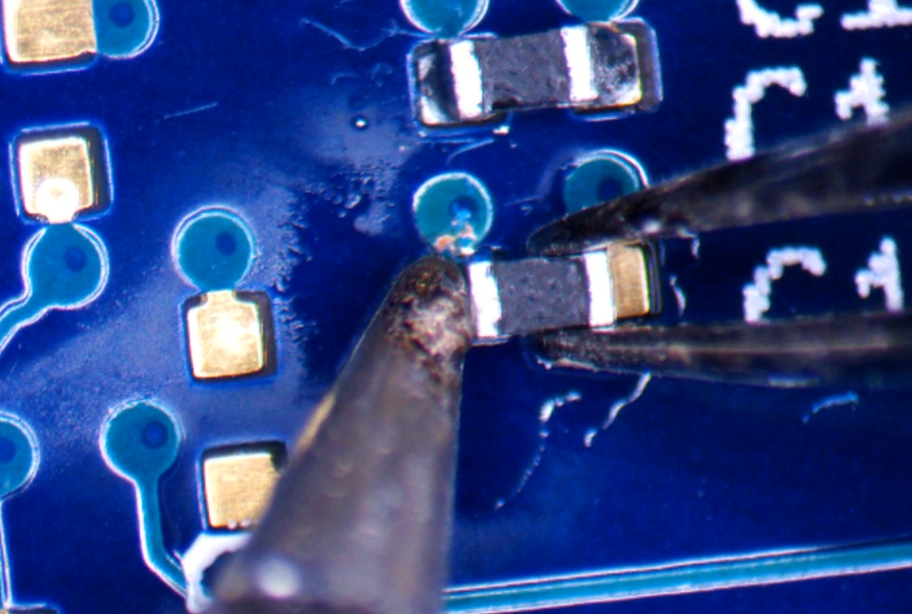
\includegraphics[height=3cm,keepaspectratio]{intro-shot.jpg}
\end{center}
\end{frame}

\begin{frame}
\frametitle{Safety concerns}
\begin{itemize}
\item Toxic heavy metals (Pb, Cd, Sb)
\item High temperatures
\item Flux smoke
\end{itemize}
\begin{center}
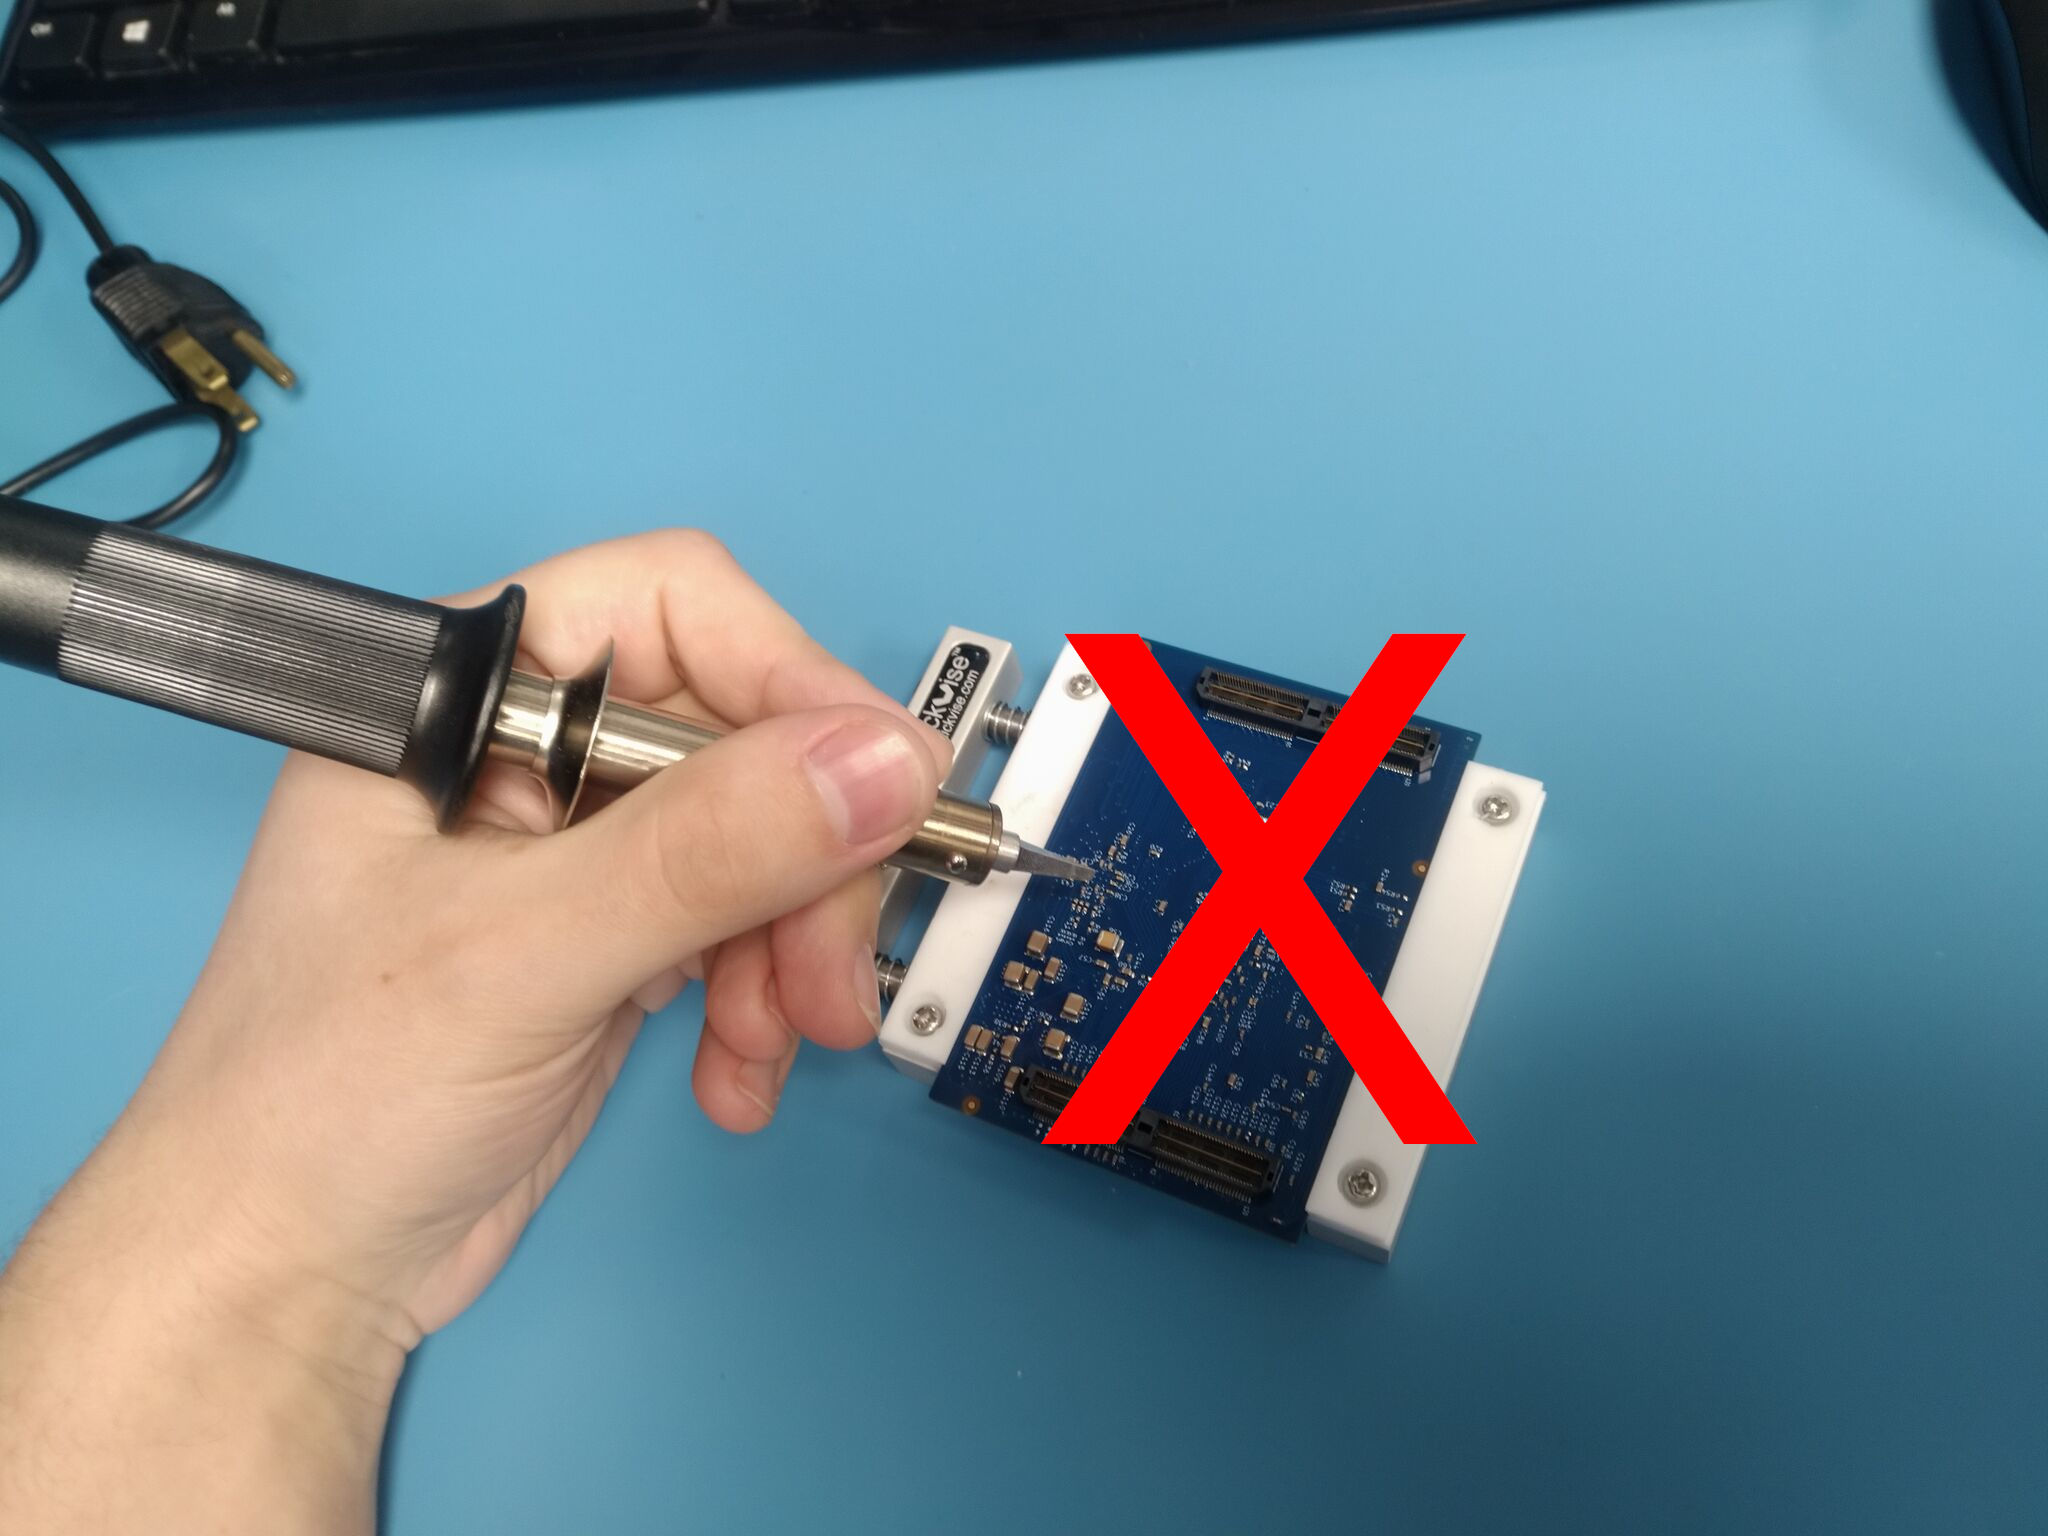
\includegraphics[width=3cm,keepaspectratio]{safety.jpg}
\end{center}
\end{frame}

\begin{frame}
\frametitle{Soldering Processes}
We can classify soldering processes by the heat source used.
\begin{itemize}
\item \textbf{Iron soldering} \\
A heated metal tip provides heat to the joint by \emph{conduction}
\item \textbf{Reflow soldering} \\
Non-contact heating using \emph{convection} or \emph{radiation} in an oven or with a hand-held tool
\end{itemize}
\end{frame}

\begin{frame}
\frametitle{Anatomy of a Soldering Iron}
\begin{itemize}
\item Insulated handle
\item Heat source
\item Tip
\end{itemize}
\begin{center}
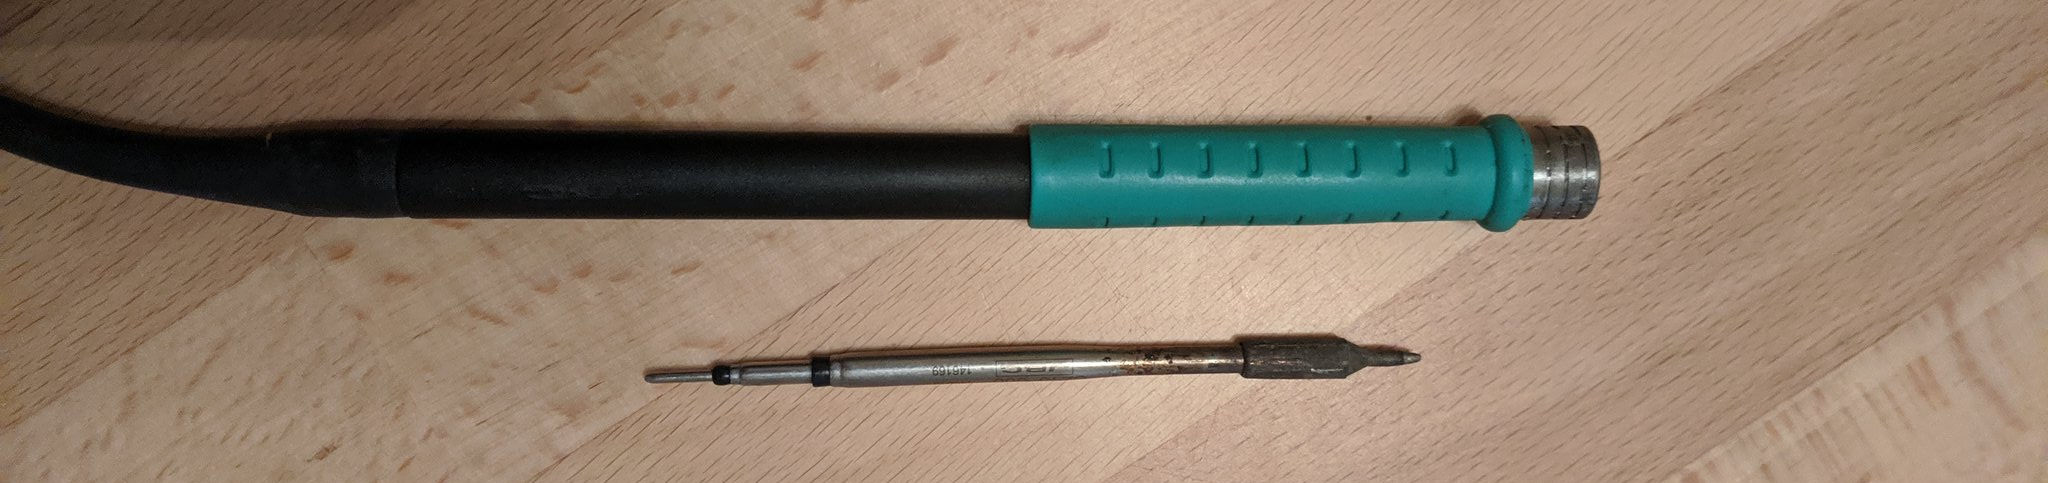
\includegraphics[width=10cm,keepaspectratio]{anatomy.jpg}
\end{center}
\end{frame}

\begin{frame}
\frametitle{Soldering Iron Heat Sources}
\begin{itemize}
\item \textbf{Combustion} \\
Portable, but poor temperature control. Rarely used.
\item \textbf{Electrical} \\
Universally used for precision electronics work.
\end{itemize}
\end{frame}

\begin{frame}
\frametitle{Soldering Iron Temperature Control}
\begin{itemize}
\item \textbf{None} \\
Lowest cost. Useless for precision work.
\item \textbf{Resistive element + sensor} \\
Most commonly used. Easily adjustable as needed.
\item \textbf{Curie point} \\
More expensive. Very stable but not adjustable.
\end{itemize}
\end{frame}

\begin{frame}
\frametitle{Solder Materials}
\begin{itemize}
\item \textbf{Sn-Pb} \\
Industry standard until early 2000s
\item \textbf{Sn-Ag-Cu (SAC)} \\
Lead free, higher melting point. Widely used.
\item \textbf{In/Bi based} \\
Various alloys with low melting point. Brittle.
\end{itemize}
\end{frame}

\begin{frame}
\frametitle{Tin Whiskers}
\begin{itemize}
\item x
\end{itemize}
\end{frame}

\begin{frame}
\frametitle{Sn-Pb Solder Alloys}
\begin{itemize}
\item Largely immune to tin whiskers
\item Midrange melting point (183C for 63/37 eutectic)
\item Banned in Europe since 2003 due to toxicity concerns
\item Still used in some medical/aerospace applications
\end{itemize}
\begin{alertblock}{Safety note}
Lead is a cumulative neurotoxin! Wash hands after handling lead-based solder.
\end{alertblock}
\end{frame}

\begin{frame}
\frametitle{SAC Solder Alloys}
\begin{itemize}
\item Sn/Ag/Cu. 3\% Ag / 0.5\% Cu is most common
\item Not eutectic, but close
\item Higher melting point (SAC305 is 217-220C)
\item Nontoxic
\item Tin whisker concerns
\end{itemize}
\end{frame}

\begin{frame}
\frametitle{Low melting point alloys}
\begin{itemize}
\item Used on heat-sensitive components (LED lighting etc)
\item 52\% In / 48\% Sn melts at 118C
\item 57\% Bi / 42\% Sn / 1\% Ag melts at 138C
\item 100\% In melts at 157C
\item Generally brittle
\end{itemize}
\end{frame}

\begin{frame}
\frametitle{PCB Surface Finishes}
\begin{itemize}
\item \textbf{None}\\
Bare copper. Corrodes rapidly, rarely used
\item \textbf{HASL} \\
Thin plating of solder. Tends to form ``humps" over pads
\item \textbf{OSP} \\
Very thin polymer layer. Short shelf life.
\item \textbf{Immersion tin/silver} \\
Thin layer of easily solderable material
\item \textbf{ENIG} \\
Typ. $5 \mu m$ Ni, $100 nm$ Au. Expensive but long shelf life.
\end{itemize}
\end{frame}

\begin{frame}
\frametitle{Intermetallic Compounds}
\begin{itemize}
\item Cu, Sn, etc are \emph{soluble} in molten solder!
\item When molten solder is applied to a surface, \emph{diffusion} takes place between the surface and solder
\item The resulting \emph{intermetallic compound} (IMC) bonds strongly to both the solder and component.
\item No IMC = no solder joint (e.g. Sn based solder on Al surface)
\item IMC is, unfortunately, more brittle than bulk solder
\end{itemize}
\end{frame}

\begin{frame}
\frametitle{Oxidation}
\begin{itemize}
\item Metals like to form oxides, esp. when heated
\item Workpieces and solder wire have ``native oxide" layer
\item Working under inert gas inhibits additional oxidation, but won't remove native oxide
\item Oxides prevent IMC formation and free flow of molten solder
\end{itemize}
\end{frame}

\begin{frame}
\frametitle{Soldering Fluxes - Function}
\begin{itemize}
\item Remove native oxide from surfaces
\item Prevent oxidation of molten solder
\item Strong reducing agents - oxidize rapidly when heated in air
\end{itemize}
\end{frame}

\begin{frame}
\frametitle{Soldering Fluxes - Types}
\begin{itemize}
\item Natural rosin vs synthetic compounds
\item Cleaning required? Hot water, alcohol, other solvent?
\item Form - Gel, liquid, foam
\end{itemize}
\begin{alertblock}{Safety note}
Long-term exposure to flux vapors can trigger allergic reactions or cause asthma. Avoid inhaling flux smoke.
\end{alertblock}
\end{frame}

\end{document}
